% --------------------------------------------
% Definição do tipo do documento e suas
% características.
% --------------------------------------------
\documentclass[
    12pt,                   % Tamanho da fonte.
    a4paper,                % Tipo de papel.
    sumario=tradicional,    % Tipo de sumário.
    brazil,                 % Linguagem principal do documento.
    oneside                 % Imprimir documento em um lado da folha.
]{abntex2}                  % Estilo do documento.

% --------------------------------------------
% Importação de configurações pessoais.
% --------------------------------------------
\usepackage{setup/packages}


%! Author = gabriel
%! Date = 5/17/21

% --------------------------------------------
% Insira o nome do(s) autor(es).
% Caso seja mais de um, insira \and entre os
% nomes de cada um.
% --------------------------------------------
\author{Gabriel Medeiros Lopes Carneiro}

% --------------------------------------------
% Insira o nome da universidade.
% --------------------------------------------
\university{Universidade Federal de Santa Catarina}

% --------------------------------------------
% Insira o nome do centro de ensino.
% --------------------------------------------
\educationcenter{Centro Tecnológico}

% --------------------------------------------
% Insira o nome do departamento de ensino.
% --------------------------------------------
\department{Departamento de Informática e Estatística}

% --------------------------------------------
% Insira o nome do curso ao qual pertence.
% --------------------------------------------
\course{Ciências da Computação}

% --------------------------------------------
% Afiliação do autor.
% -------------------------------------------- 
\affil{\printuniversity \\
        \printeducationcenter \\
        \printdepartment \\
        \printcourse}

%! Author = gabriel
%! Date = 5/17/21

% --------------------------------------------
% Insira o título do trabalho.
% --------------------------------------------
\title{Título}
% --------------------------------------------
% Caso o trablalho tenha subtítulo, descomente
% a linha abaixo.
% OBS.: NÃO APAGAR ":~" irá desconfigurar o arquivo.
% --------------------------------------------
\subtitle{:~Subtítulo (se houver)}

% --------------------------------------------
% Insira o tipo de trabalho do documento.
% --------------------------------------------
\worktype{Tipo do trabalho}

% --------------------------------------------
% Insira o local de apresentação do documento.
% --------------------------------------------
\local{Florianópolis, SC}

% --------------------------------------------
% Define a data do documento. Por padrão mostra
% apenas o ano, caso queira a data completa,
% substitua por \today.
% --------------------------------------------
\date{\the\year}

% --------------------------------------------
% Caso o trabalho possua um orientador,
% comente a linha abaixo.
% --------------------------------------------
\orientador[Professor:]{Nome completo do professor}

% --------------------------------------------
% Caso o documento possua um orientador,
% descomente a linha abaixo.
% --------------------------------------------
%\orientador{Nome completo do orientador}

% --------------------------------------------
% Caso o documento possua um coorientador,
% descomente a linha abaixo.
% --------------------------------------------
%\coorientador{Nome completo do coorientador}

% --------------------------------------------
% Substituir '[mestre/doutor] em título obtido'
% pelo grau adequado.
% --------------------------------------------
%\formation{mestre/doutor em título obtido}

% --------------------------------------------
% Substituir nome do curso pelo nome do curso.
% --------------------------------------------
%\program{Programa de Pós-Graduação em nome do curso}

% --------------------------------------------
% Caso precise do preâmbulo do documento,
% descomente as linhas abaixo. Ele deve conter,
% o tipo do documento, o objetivo, o nome da
% instituição e a área de concentração.
% --------------------------------------------
%\preambulo{
%    \printworktype~ submetida ao
%    \printprogram~ da \printuniversity~
%    para a obtenção do título de \printformation.
%}

% --------------------------------------------
% Definição de cores de hyperlinks
% e formatações do pdf.
% --------------------------------------------
\hypersetup{
    colorlinks=true,
    linkcolor=black,
    filecolor=magenta,
    urlcolor=blue,
    citecolor=black,
    pdfauthor=\theauthor,
    pdftitle=\thetitle,
    bookmarksopen=true,
}

% --------------------------------------------
% Início do documento.
% --------------------------------------------
% Aqui devem ser inseridas todas informações.
% --------------------------------------------
\begin{document}
    % --------------------------------------------
    % Inserção dos elementos pré-textuais.
    % --------------------------------------------
    % Capa, folha de rosto, ficha catalográfica,
    % errata, folha de aprovação, dedicatória,
    % agradecimentos, epígrafe, resumos,
    % lista de ilustrações, lista de tabelas,
    % lista de abreviaturas e siglas,
    % lista de símbolos e sumário.
    % --------------------------------------------
    %! Author = gabriel
%! Date = 5/17/21

% Logo da UFSC
%\begin{figure}
%    
\includegraphics[scale=0.2]{logo-ufsc}
%    \centering
%    \label{fig:logo-ufsc}
%\end{figure}

% Geração de Título

% --------------------------------------------
% Para usar título padrão latex, descomente
% a linha abaixo.
% --------------------------------------------
%\maketitle

% TODO: melhorar capa


% --------------------------------------------
% Geração da capa.
% --------------------------------------------
\printcoverufsc
%\printcover

% --------------------------------------------
% Geração da folha de rosto.
% --------------------------------------------
\printtitlepage

% --------------------------------------------
% Resumo do documento de acordo com padrões
% Latex. Caso queira de acordo com a ABNT,
% comente as linhas abaixo.
% --------------------------------------------
%\begin{abstract}
%    Write here.
%\end{abstract}

% --------------------------------------------
% Comentar linhas abaixo para não ter um
% resumo de acordo com a ABNT.
% --------------------------------------------
\begin{resumo}
    A bolsa de iniciação científica teve como foco de estudo computação quântica.
    Durante o período, duas linguagens de programação quântica foram estudadas, sendo elas Qiskit e Ket.
    Além disso, os principais algoritmos quânticos foram vistos, como, por exemplo, o algoritmo de busca de Grover, a estimativa de fase, busca de ordem, entre outros.
    Com os conhecimentos adquiridos também foi possível participar de um projeto de extensão relacionado a um simulador quântico.
\end{resumo}
\newpage

% --------------------------------------------
% Caso seja necessário um resumo em inglês,
% descomentar linhas abaixo.
% --------------------------------------------
%\begin{resumo}[Abstract]
%    Escreva o resumo em inglês aqui.
%\end{resumo}
%\newpage

% --------------------------------------------
% Lista de Figuras.
% --------------------------------------------
\listoffigures*
\newpage

% --------------------------------------------
% Lista de Tabelas.
% --------------------------------------------
%\listoftables*
%\newpage

% --------------------------------------------
% Geração do Sumário.
% --------------------------------------------
\tableofcontents*

    % --------------------------------------------
    % Inserção dos elementos textuais.
    % --------------------------------------------
    % Aqui devem ser inseridos todos os capítulos
    % e/ou seções do trabalho.
    % --------------------------------------------
    % --------------------------------------------
% Aqui você deve organizar as seções.
% --------------------------------------------
\chapter{Introdução}\label{ch:introducao}

\section{Motivação}\label{sec:Motivacao}
% --------------------------------------------
% Aqui você deve escrever o texto.
% --------------------------------------------
Escreva aqui.

\section{Justificativas}\label{sec:Justificativas}
% --------------------------------------------
% Aqui você deve escrever o texto.
% --------------------------------------------
Escreva aqui.\cite{einstein}

\section{Objetivos}\label{sec:Objetivos}
% --------------------------------------------
% Aqui você deve organizar as subsubseções.
% --------------------------------------------
\subsection{Objetivo Geral}\label{subsec:objetivo-geral}
% --------------------------------------------
% Aqui você deve escrever o texto.
% --------------------------------------------
Escreva aqui.

\subsection{Objetivos Específicos}\label{subsec:objetivos-especificos}
% --------------------------------------------
% Aqui você deve escrever o texto.
% --------------------------------------------

    \chapter{Computação Quântica}\label{ch:computacao-quantica}

\section{Breve Histórico}\label{sec:breve-historico}

No início do século XX os cientistas enfrentavam um grande problema, que
era explicar o comportamento da radiação emitida por um corpo negro.
A solução desse problema levou ao surgimento da Mecânica Quântica, que
segundo a hipótese de Max Planck ``a radiação só pode ser emitida ou
absorvida por um corpo negro em quantidades múltiplas inteiras de
\(hf\)'', em que \(h \approx 6,62 \cdot 10^{-34} J \cdot s\) é a
constante de Planck e \(f\) é a frequência de radiação.
A quantização da energia e de outras grandezas na escala atômica foi importante para
explicar uma série de outros fenômenos, como por exemplo o efeito
fotoelétrico e o espectro da radiação emitida por átomos e moléculas.
O desenvolvimento da Mecânica Quântica nos permitiu compreender melhor o
comportamento da matéria na escala microscópica, nesse caso particular,
os materiais semicondutores, que permitiram a criação do transistor.
Os transistores substituíram as válvulas usadas nos primeiros computadores
digitais a partir de 1955.
É importante notar que a lógica usada para realizar as operações computacionais nos nossos notebooks, PCs, tablets e smartphones é a lógica booleana, ou seja, uma lógica clássica que
envolve operações como AND, OR e NOT sobre os bits 0 e 1.
Devido a sua grande capacidade de cálculo e armazenamento, os computadores são
fundamentais para o desenvolvimento de qualquer sociedade moderna.
Essa é a chamada primeira revolução quântica.

Um dos grandes impulsionadores da computação quântica foi o físico
Richard Feynman, que no início da década de 80 sugeriu o uso de
computadores quânticos para simular sistemas quânticos.
A percepção de Feynman baseia-se no fato de que o número de configurações possíveis nos
sistemas quânticos cresce de maneira exponencial com o número de entes
(spins, elétrons, átomos, \ldots) considerados, tornando-se proibitivo para
a memória dos computadores atuais guardar tanta informação mesmo para um
número pequeno (\(< 100\)) de partículas.

Na década seguinte, os primeiros algoritmos quânticos começaram a
surgir, dentre eles, os que mais se destacaram foram o algoritmo de
busca de Grover e o de fatoração de Shor.
Este último algoritmo foi provavelmente um dos grandes responsáveis pelo desenvolvimento da
computação quântica, já que é capaz de encontrar os fatores primos \(p\)
e \(q\) que multiplicados resultavam em um número inteiro
\(N = p \cdot q\) em uma escala de tempo que cresce polinomialmente com
o tamanho do número \(N\).
Ou seja, a base do sistema de segurança RSA, amplamente usado para realizar transações bancárias no mundo todo, pode estar comprometida a partir da existência de computadores quânticos de
larga escala.

A partir da segunda década do século XXI, não apenas a computação
quântica, mas outras áreas como criptografia quântica, sensores
quânticos e simulação quântica tem recebido forte atenção não apenas do
setor acadêmico, mas também do setor industrial.
Dessa forma, tem-se observado o rápido desenvolvimento das chamadas tecnologias quânticas, o
que configura a segunda revolução quântica, uma vez que a lógica por
trás dos processos é de natureza quântica.

\section{Desenvolvimento Atual}\label{sec:desenvolvimento-atual}

A Computação Quântica ainda está em fase de amadurecimento, mas já
mostra o seu grande potencial para resolver problemas práticos, além do
algoritmo de fatoração de Shor e de busca de Grover, tais como problemas
de otimização, machine learning, logística, química quântica, finanças,
álgebra linear, entre outros.
Nos últimos cinco anos, grandes empresas como Google, IBM, Amazon e Microsoft intensificaram ainda mais os seus investimentos no setor, além de vários governos de diversos países da
América do Norte, Europa, Oceania e Ásia.
Um dos grande temores em relação ao computadores quânticos está relacionado à segurança da
informação, que afeta não apenas as transações bancárias, mas toda e
qualquer transmissão de informação sigilosa, incluindo a militar,
naturalmente.
Tentativas de barrar possíveis ataques por computadores
quânticos incluem a criptografia pós-quântica, que apesar do nome, se
baseia em métodos criptográficos clássicos.

Para quem estiver interessado em aprender computação quântica, vale
lembrar que algumas empresas disponibilizam computadores quânticos
reais, simuladores, kits e linguagens para desenvolvimento de algoritmos
ao público geral.
Por exemplo, é possível acessar gratuitamente o kit de desenvolvimento quântico criado pela IBM
(\href{https://qiskit.org/}{Qiskit}) e rodar algoritmos em alguns dos
seus computadores quânticos com poucos qubits.
Através deste projeto será possível programar em um simular quântico de até 30 qubits de
maneira gratuita, através da linguagem
\href{https://quantumket.org/}{Ket} e do simulador
\href{https://qubox.ufsc.br/qubox.html}{QuBOX}.

\section{O que é um qubit?}\label{sec:qubit}

O qubit (\textbf{qu}antum + \textbf{bit}) é um bit quântico.
O bit clássico sempre está em um dos possíveis estados 0 ou 1, já um qubit
pode estar em ambas configurações simultaneamente.
Chamamos esse fenômeno de {superposição}.
Para representar um qubit utilizamos a notação Dirac ou “braket”:

\[\begin{aligned}
\left | \psi \right \rangle = \begin{bmatrix} a \\ b \end{bmatrix} = a \left| 0 \right \rangle + b \left| 1 \right \rangle
\end{aligned}\]

em que \(a\) e \(b\) são {amplitudes de probabilidade} (números
complexos), de modo que

\begin{gather*}
    |a|^2 \text{ representa a probabilidade de após uma medida encontrar o sistema no estado}
\left| 0 \right\rangle\\
    |b|^2 \text{ representa a probabilidade de após uma medida encontrar o sistema no estado}
\left| 1 \right\rangle\\
\end{gather*}

Como a probabilidade total deve somar \(100\%\), temos que a {condição
de normalização} para o estado \(\left| \psi \right\rangle\) é
\(|a|^2 + |b|^2 = 1\).

\subsection{Esfera de Bloch}\label{subsec:esfera-de-bloch}

Os estados de um qubit podem ser representados por meio de pontos em uma
superfície esférica de raio unitário, utilizando o sistema de
coordenadas esféricas.
Para isso, é preciso parametrizar o estado do qubit
\(\left| \psi \right\rangle = a \left| 0 \right\rangle + b \left| 1 \right\rangle\)
da seguinte forma

\[\left| \psi \right\rangle = \cos\left(  \dfrac{\theta}{2} \right) \left| 0 \right\rangle + e^{i\phi} \sin\left( \dfrac{\theta}{2} \right) \left| 1 \right\rangle \text{ tal que } \theta \in [0, \pi], \phi \in [0, 2\pi)\]

Agora, utilizando \(\theta\) e \(\phi\) no sistemas de coordenadas
esféricas, tem-se a Esfera de Bloch.
Todos os estados acessíveis a um qubit podem ser representados utilizando-se \autoref{fig:esfera-bloch}.

\begin{figure}[!htp]
    \centering
    \includesvg[width=0.8\textwidth,height=\textheight]{utils/Bloch_Sphere.svg}
    \caption{Representação de um qubit na Esfera de Bloch.}
    \label{fig:esfera-bloch}
\end{figure}

\subsection{Representação de 2 ou mais qubits}\label{subsec:repr}

Existem diversas formas de se representar um sistema de 2 qubits, seguem
algumas equivalências:

\[\left| \psi_0 \right\rangle \otimes \left| \psi_1 \right\rangle = \left| \psi_0 \right\rangle \left| \psi_1 \right\rangle = \left| \psi_0 \psi_1 \right\rangle\]

em que \(\otimes\) é produto tensorial de \(\psi_0\) com \(\psi_1\).
Seja

\[\begin{aligned}
\left| \psi_0 \right\rangle \otimes \left| \psi_1 \right\rangle
= \begin{bmatrix} a_0 \\ a_1 \end{bmatrix} \otimes \begin{bmatrix} b_0 \\ b_1 \end{bmatrix}
= \begin{bmatrix} a_0 b_0 \\ a_0 b_1 \\ a_1 b_0 \\ a_1 b_1 \end{bmatrix}
\end{aligned}\]

De forma análoga, é possível representar sistemas de \(n\) qubits como

\[\left| \psi_0 \right\rangle \otimes \left| \psi_1 \right\rangle \otimes \dots \otimes \left| \psi_n \right\rangle
= \left| \psi_0 \right\rangle \left| \psi_1 \right\rangle \dots \left| \psi_n \right\rangle
= \left| \psi_0 \psi_1 \dots \psi_n \right\rangle\]

Como será mostrado na \autoref{sec:emaranhamento}, a superposição de estados desse tipo pode levar ao emaranhamento.

\section{Etapas de um Algoritmo Quântico}\label{sec:etapas-quanticas}

\begin{figure}[!htp]
    \centering
    \includesvg[width=1\textwidth,height=\textheight]{utils/diagrama.svg}
    \caption{Etapas básicas de um algoritmo quântico}
    \label{fig:etapas-alg}
\end{figure}

De forma geral, é possível separar um algoritmo quântico em quatro etapas, como mostra a \autoref{fig:etapas-alg}.

\begin{enumerate}
\tightlist
\item
  \textbf{Preparação}: aqui cada qubit é inicializado em algum estado,
  geralmente em \(\left| 0 \right\rangle\).
\item
  \textbf{Evolução}: nessa parte o algoritmo é de fato aplicado, através
  das portas lógicas quânticas.
\item
  \textbf{Medida}: após a aplicação das portas, é necessário medir os
  qubits, para se ter o resultado do circuito.
\item
  \textbf{Pós-processamento}: finalmente, nessa etapa o resultado obtido
  deve ser interpretado de acordo com o contexto.
\end{enumerate}

\section{Comparação com Computação Clássica}\label{sec:compare}

\subsection{Entradas e Saídas}\label{subsec:entradas-e-saidas}

\begin{itemize}
\tightlist
\item
  \textbf{Clássica}: portas podem ter diferentes números de bits
  entrando e saindo.
\end{itemize}

\textbf{Exemplo}

A porta AND possui dois ou mais bits de entrada e apenas um de saída.

\begin{figure}
    \centering
    \includesvg[width=0.15\textwidth,height=\textheight]{utils/gates/and.svg}
    \caption{Representação da porta AND.}
    \label{fig:and}
\end{figure}

\begin{itemize}
\tightlist
\item
  \textbf{Quântica}: portas possuem mesmo número de qubits na entrada e
  na saída.
\end{itemize}

\subsection{Reversibilidade}\label{subsec:reversibilidade}

\begin{itemize}
\tightlist
\item
  \textbf{Clássica}: a maioria das portas clássicas não são reversíveis,
  isto é, dado uma saída não conseguimos identificar quais foram as
  entradas.
\end{itemize}

\textbf{Exemplo}

Na porta OR de dois bits podemos obter 1 como saída em três casos.

\[\begin{aligned}
\begin{array}{cc|c}
    X & Y & X \text{ OR } Y \\
    0 & 0 & 0 \\
    0 & 1 & 1 \\
    1 & 0 & 1 \\
    1 & 1 & 1 \\
\end{array}
\end{aligned}\]

Sabendo que a saída foi 1 não é possível identificar qual/quais bits
eram 1.

\begin{itemize}
\tightlist
\item
  \textbf{Quântica}: seus circuitos são reversíveis, isso ocorre, pois,
  seus operadores são unitários.
\end{itemize}

\textbf{Observação}

Embora a evolução temporal seja reversível durante o processamento da
informação no circuito quântico, a medição dos qubits é um processo
irreversível.

\section{Portas Lógicas Quânticas}\label{sec:portas-quanticas}

As portas lógicas quânticas são operações {unitárias} que ao atuar em um
estado inicial levam para outro estado final, ou seja, funcionam como
rotações na esfera de Bloch.
A seguir, alguns exemplos de portas lógicas quânticas que atuam sobre um qubit.

\subsection{Porta X}\label{subsec:porta-x}

Essa porta é o equivalente a porta NOT da computação clássica.

Matriz

\[\begin{aligned}
X = \sigma_x =
\begin{bmatrix}
    0 & 1 \\
    1 & 0
\end{bmatrix}
\end{aligned}\]

Comportamento

\[\begin{aligned}
\begin{matrix}
    X \left| 0 \right\rangle &=& \left| 1 \right\rangle \\
    X \left| 1 \right\rangle &=& \left| 0 \right\rangle
\end{matrix}
\end{aligned}\]

Símbolo

\begin{figure}[!htp]
    \centering
    \includesvg[width=0.15\textwidth,height=\textheight]{utils/gates/xgate.svg}
    \caption{Representação da porta X.}
    \label{fig:xgate}
\end{figure}

ou ainda

\begin{figure}[!htp]
    \centering
    \includesvg[width=0.15\textwidth,height=\textheight]{utils/gates/targgate.svg}
    \caption{Outra representação da porta X.}
    \label{fig:targ-gate}
\end{figure}


\subsection{Porta Y}\label{subsec:porta-y}

Matriz

\[\begin{aligned}
Y = \sigma_y =
\begin{bmatrix}
    0 & -i \\
    i & 0
\end{bmatrix}
\end{aligned}\]

Comportamento

\[\begin{aligned}
\begin{matrix}
    Y \left| 0 \right\rangle &=& i\left| 1 \right\rangle \\
    Y \left| 1 \right\rangle &=& -i\left| 0 \right\rangle
\end{matrix}
\end{aligned}\]

Símbolo

\begin{figure}[!htp]
    \centering
    \includesvg[width=0.15\textwidth,height=\textheight]{utils/gates/ygate.svg}
    \caption{Representação da porta Y.}
    \label{fig:ygate}
\end{figure}


\subsection{Porta Z}\label{subsec:porta-z}

A porta Z introduz uma fase relativa de \(\pi\) entre os estados da base
computacional.

Matriz

\[\begin{aligned}
Z = \sigma_z =
\begin{bmatrix}
    1 & 0 \\
    0 & -1
\end{bmatrix}
\end{aligned}\]

Comportamento

\[\begin{aligned}
\begin{matrix}
    Z \left| 0 \right\rangle &=& \left| 0 \right\rangle \\
    Z \left| 1 \right\rangle &=& -\left| 1 \right\rangle
\end{matrix}
\end{aligned}\]

Símbolo

\begin{figure}[!htp]
    \includesvg[width=0.15\textwidth,height=\textheight]{utils/gates/zgate.svg}
    \caption{Representação da porta Z.}
    \label{fig:zgate}
\end{figure}

\subsection{Porta Hadamard}\label{subsec:porta-hadamard}

Essa porta gera uma superposição dos estados da base computacional.

Matriz

\[\begin{aligned}
H = \dfrac{1}{\sqrt{2}}
\begin{bmatrix}
    1 & 1 \\
    1 & -1
\end{bmatrix}
\end{aligned}\]

Comportamento

\[\begin{aligned}
\begin{matrix}
    H \left| 0 \right\rangle &=& \dfrac{1}{\sqrt{2}} \left( \left| 0 \right\rangle + \left| 1 \right\rangle \right) &=& \left| + \right\rangle \\
    H \left| 1 \right\rangle &=& \dfrac{1}{\sqrt{2}} \left( \left| 0 \right\rangle - \left| 1 \right\rangle \right) &=& \left| - \right\rangle \\
\end{matrix}
\end{aligned}\]

Símbolo

\begin{figure}[!htp]
    \centering
    \includesvg[width=0.15\textwidth,height=\textheight]{utils/gates/hgate.svg}
    \caption{Representação da porta H.}
    \label{fig:hgate}
\end{figure}


\subsection{Portas Controladas}\label{subsec:portas-controladas}

Para se fazer computação quântica universal, ou seja, realizar todas as
transformações unitárias desejadas entre os qubits de entrada e saída em
um algoritmo, é necessário realizar operações que façam dois ou mais
qubits interagirem entre si.
Tais portas podem envolver um qubit de controle e o outro como alvo, sendo possível generalizá-la para
múltiplos qubits de controle e de alvo.
Segue o exemplo para porta controlada X, ou CNOT, com um controle e um alvo.

Matriz

\[\begin{aligned}
\text{CNOT} =
\begin{bmatrix}
    1 & 0 & 0 & 0 \\
    0 & 1 & 0 & 0 \\
    0 & 0 & 0 & 1 \\
    0 & 0 & 1 & 0
\end{bmatrix}
\end{aligned}\]

Comportamento

\[\begin{aligned}
\begin{matrix}
    \text{CNOT} \left| 00 \right\rangle &=& \left| 00 \right\rangle \\
    \text{CNOT} \left| 01 \right\rangle &=& \left| 01 \right\rangle \\
    \text{CNOT} \left| 10 \right\rangle &=& \left| 11 \right\rangle \\
    \text{CNOT} \left| 11 \right\rangle &=& \left| 10 \right\rangle
\end{matrix}
\end{aligned}\]

Símbolo

\begin{figure}[!htp]
    \centering
    \includesvg[width=0.15\textwidth,height=\textheight]{utils/gates/cxgate.svg}
    \caption{Representação da porta X-controlada.}
    \label{fig:cnot}
\end{figure}

ou ainda

\begin{figure}[!htp]
    \centering
    \includesvg[width=0.15\textwidth,height=\textheight]{utils/gates/ctarggate.svg}
    \caption{Outra representação da porta X-controlada.}
    \label{fig:cnot2}
\end{figure}


\section{Emaranhamento}\label{sec:emaranhamento}

Estados emaranhados são aqueles que não podem ser escritos como produto
tensorial de estados de 1 qubit, ou seja, não é possível separá-los.
Os mais conhecidos são os estados de Bell, os quais envolvem apenas 2
qubits, sendo dados por:

\[\begin{aligned}
\begin{matrix}
\left| \beta_{00} \right\rangle &=& \left| \Phi^+ \right\rangle &=& \dfrac{1}{\sqrt{2}} \left( \left| 00 \right\rangle + \left| 11 \right\rangle \right) \\
\left| \beta_{01} \right\rangle &=& \left| \Phi^- \right\rangle &=& \dfrac{1}{\sqrt{2}} \left( \left| 00 \right\rangle - \left| 11 \right\rangle \right) \\
\left| \beta_{10} \right\rangle &=& \left| \Psi^+ \right\rangle &=& \dfrac{1}{\sqrt{2}} \left( \left| 01 \right\rangle + \left| 10 \right\rangle \right) \\
\left| \beta_{11} \right\rangle &=& \left| \Psi^- \right\rangle &=& \dfrac{1}{\sqrt{2}} \left( \left| 01 \right\rangle - \left| 10 \right\rangle \right)
\end{matrix}
\end{aligned}\]

Os estados emaranhados são apontados como sendo os responsáveis por fazer
não apenas a computação quântica mais veloz do que a computação
clássica, mas também permitem aumentar a precisão de medidas de
observáveis físicos e realizar comunicação de forma segura.

\subsection{Criando um Estado de Bell}\label{subsec:criando-um-estado-de-bell}

Com o conceito de emaranhamento explicado, resta saber como criá-lo.
Como exemplo, o estado \(\left| \beta_{00} \right\rangle\) será criado, na \autoref{fig:estados-bell} temos o circuito para isso e em \autoref{lst:estado-bell} o código para o mesmo usando Ket.

\begin{figure}
    \centering
    \includesvg[width=0.4\textwidth,height=\textheight]{utils/bell_state.svg}
    \caption{Circuito para criar um estado de Bell.}
    \label{fig:estados-bell}
\end{figure}

\begin{listing}[!htb]
\begin{minted}{python}
q0, q1 = quant(2)   # cria dois qubits
H(q0)               # aplica a porta de Hadamard no qubit 0
ctrl(q0, X, q1)     # aplica a porta X no qubit 1, com o qubit 0 como controle
\end{minted}
\caption{Criando um estado de Bell em Ket.}
\label{lst:estado-bell}
\end{listing}

Seja \(\left| \psi \right\rangle = q_0 \otimes q_1\).
Após a aplicação da porta de Hadamard, teremos
\(q_0 = \dfrac{1}{\sqrt{2}} \left( \left| 0 \right\rangle + \left| 1 \right\rangle \right)\),
conforme visto anteriormente.
Logo,

\[\begin{aligned}
\begin{matrix}
    \left| \psi \right\rangle &=&    \dfrac{1}{\sqrt{2}} \left( \left| 0 \right\rangle + \left| 1 \right\rangle \right) \otimes \left| 0 \right\rangle \\
    &=& \dfrac{1}{\sqrt{2}} \left( \left| 00 \right\rangle + \left| 10 \right\rangle\right)
\end{matrix}
\end{aligned}\]

Na sequência, temos uma porta CNOT, com o qubit 0 como controle e o qubit 1 como alvo.
Gerando a seguinte situação

\[\begin{aligned}
\begin{matrix}
    \left| \psi \right\rangle &=&        \text{CNOT} \left[ \dfrac{1}{\sqrt{2}} \left( \left| 00 \right\rangle + \left| 10 \right\rangle\right) \right] \\
    &=& \dfrac{1}{\sqrt{2}} \left( \text{CNOT} \left| 00 \right\rangle + \text{CNOT} \left| 10 \right\rangle \right) \\
    &=& \dfrac{1}{\sqrt{2}} \left( \left| 00 \right\rangle + \left| 11 \right\rangle \right) \\
    &=& \left| \beta_{00} \right\rangle
\end{matrix}
\end{aligned}\]

Portanto, com apenas duas portas é possível gerar uma situação de
emaranhamento.

    \chapter{Desenvolvimento}\label{ch:desenvolvimento}

\section{Qiskit}\label{sec:qiskit}

Inicialmente, foi planejado utilizar o material didático fornecido pelo Qiskit para o aprendizado de conceitos básicos.
Qiskit é uma ferramenta de desenvolvimento quântico criado pela IBM que permite o uso de simuladores e computadores quânticos no nível de pulsos, circuitos e outros tipos de aplicações.
Atualmente, é a ferramenta mais popular.

Com o decorrer dos estudos, alguns problemas foram identificados.
O primeiro foi referente aos cursos introdutórios, os quais não apresentavam aprofundamento necessário para se compreender os assuntos, em geral, faltavam mais explicações sobre conceitos físicos e matemáticos por trás.
Esse problema começou a ser parcialmente resolvido com a atualização dos cursos no final de 2021, mas as mudanças chegavam a passos lentos, muitas vezes as alterações feitas já estavam defasadas em relação ao desenvolvimento atual da ferramenta.
Isso se deve ao fato da ferramenta ser de código aberto e possuir uma comunidade muito ativa, recebendo várias alterações e melhorias com frequência.
Além disso, por se tratar de uma tecnologia relativamente nova e devido a essas frequentes atualizações, a ferramenta não possui um longo período de estabilidade entre versões, algo que torna códigos obsoletos rapidamente.

Outro problema encontrado foi com o acesso aos computadores quânticos da IBM.
Mesmo com a licença de estudante, os computadores disponíveis são poucos e possuem poucos qubits, tornando inviável usá-los para experimentos que exijam mais qubits.
Recentemente, a IBM retirou o computador que possuía mais qubits da licença de estudantes, dificultando ainda mais os estudos.
A alternativa, portanto, foi usar os simuladores quânticos disponíveis, mas logo se tornou enviável devido às constantes atualizações.

\section{Material Básico}\label{sec:material-basico}

Após os problemas enfrentados com o material do Qiskit, passou-se a usar\cite{giovani} como fonte de estudos.
Esse material foi criado por \citeauthor{giovani} durante seu TCC em Engenharia Eletrônica e facilitou, e muito, o aprendizado.
Ao ler o material passa-se por uma revisão de algebra linear, com foco em computação quântica, para então se ter uma introdução à mecânica quântica e computação quântica, algo que os tutorias do Qiskit não fornecem.

\section{Tópicos Avançados}\label{sec:topicos-avancados}

Após consolidar uma base suficientemente forte com a leitura de\cite{giovani}, os livros\cite{nielsen_chuang_2010, thomas-wong} foram usados para aprofundar o conhecimento em tópicos mais avançados.
O primeiro é um clássico no assunto, mostrando conceitos fundamentais, funcionamento de computadores quânticos, principais algoritmos quânticos e mais.
Já o segundo é mais recente, trazendo explicação menos densa do conteúdo ele passa por conceitos fundamentais da computação clássica e trazendo alguns comparativos entre as diferentes formas de computação.

\section{Ket}\label{sec:ket}

Ket é uma linguagem de programação embarcada em Python, projetada para facilitar o desenvolvimento de aplicações híbridas clássica-quântica.
Ket é um projeto de código aberto derivado do trabalho de mestrado de \citeauthor{ket} no Programa de Pós-Graduação em Ciência da Computação (PPGCC) da UFSC.

Essa linguagem fornece uma grande facilidade na implementação de portas lógicas quânticas, principalmente nas controladas.
Fazendo uma comparação com o Qiskit, ela é mais estável, porém não possui tantos recursos, visto que apenas o criador desenvolve a linguagem.

\section{QuBOX}\label{sec:qubox}

Com o conteúdo aprendido, foi possível participar do projeto de extensão “Simulador quântico portátil para a linguagem de programação Ket com fins educacionais e de pesquisa”, registrado no SIGPEX sob o número 202123813 e feito em uma parceria entre a startup Quantuloop e o Grupo de Computação Quântica — UFSC.
O projeto tem o objetivo de promover a computação quântica e auxiliar no desenvolvimento de novos algoritmos, métodos e aplicações quânticas.
O público alvo são alunos e professores da educação básica ao ensino superior interessados em pesquisar, aprender e ensinar computação quântica.
Além de todos os interessados em computação quântica.

Através desse projeto é possível programar em um simulador quântico de até 30 qubits de maneira gratuita, através da linguagem \href{https://quantumket.org/}{Ket} e do simulador \href{https://qubox.ufsc.br/qubox.html}{QuBOX}.
Para o projeto, foi feito um resumo sobre \href{https://qubox.ufsc.br/qc.html}{Computação Quântica} e informações e tutoriais sobre \href{https://qubox.ufsc.br/algoritmos/index.html}{algoritmos quânticos}.

    \chapter{Algoritmos Quânticos}\label{ch:algoritmos-quanticos}

Alguns dos principais algoritmos quânticos foram estudados, esses algoritmos serviram de base para vários outros, por isso foram escolhidos.

\section{Algoritmo de Busca de Grover}\label{sec:algoritmo-de-busca-de-grover}

Aqui será abordado como implementar o algoritmo quântico de Grover para
resolver o problema da busca em base de dados desordenada, o qual é mais
eficiente que as soluções clássicas.

\subsection{Problema}\label{subsec:problema}

O problema pode ser resumido em encontrar um determinado elemento dado
uma lista desordenada de tamanho \(2^n\).
Para isso, deve ser criada uma função booleana \(f: \{0, 1\}^n \to \{0, 1\}\), a qual só sinalize `1'
para o elemento desejado.

\[\begin{aligned}
f(x) =  \begin{cases}
            0, x \ne x_0 \\
            1, x = x_0
        \end{cases}
\end{aligned}\]

\textbf{Observação}

Cada elemento da lista será codificado em um estado da base
computacional \(\left| i \right\rangle, i = \{0, \dots, 2^n - 1\}\).

\subsection{Oráculo}\label{subsec:oraculo}

Um oráculo faz o mesmo que a função booleana descrita anteriormente.
Existem dois tipos de oráculos, XOR e os de fase, nesse problema será
utilizado o de fase.

\subsubsection{Oráculo de Fase}\label{subsubsec:oraculo-de-fase}

O oráculo de fase introduzirá uma fase de \(\pi\), ou seja, multiplicará
por \(-1\).

\begin{itemize}
\tightlist
\item
  Exemplo: dado
  \(\left| \psi \right\rangle = \dfrac{1}{\sqrt{2}}\left( \left| 0 \right\rangle + \left| 1 \right\rangle\right)\).
  Se o oráculo for usado para marcar o estado
  \(\left| 1 \right\rangle\), o resultado será
  \(O(\left| \psi \right\rangle) = \dfrac{1}{\sqrt{2}}\left( \left| 0 \right\rangle - \left| 1 \right\rangle\right)\).
\end{itemize}

\subsection{Algoritmo}\label{subsec:algoritmo}

O primeiro passo consiste em aplicar a porta de Hadamard em todos os
qubits para se conseguir uma superposição com pesos iguais.

\[H^{\otimes n}\left|0\right\rangle^{\otimes n}.\]

Após isso é preciso aplicar \(G\) (operador de Grover) \(k\) vezes, em que \(G\)
representa a seguinte sequência de passos:

\begin{enumerate}
\def\labelenumi{\arabic{enumi}.}
\item
  Aplicar o oráculo de fase para o estado desejado;
\item
  Aplicar a porta de Hadamard em todos os qubits;
\item
  Aplicar o operador \(2 \left| 0 \right\rangle \left\langle 0 \right| - I\);
  Na notação utilizada aqui \(\left| 0 \right\rangle\) representa \(\left| 0 \right\rangle^{\otimes n}\).
\item
  Aplicar a porta de Hadamard em todos os qubits.
\end{enumerate}

\subsubsection{Notação Auxiliar}\label{subsubsec:notacao-auxiliar}

\[\begin{aligned}
\begin{matrix}
\mathbb{B}_n: \text{conjunto de todas as palavras de n bits}. \\
\mathbb{M}: \text{conjunto de todos itens desejados}. \\
N = 2^n
\begin{cases}
n: \text{número de qubits}. \\
N: \text{número de itens}.
\end{cases} \\
M: \text{número de itens desejados (usaremos } M = 1). \\
\left| \alpha \right\rangle \coloneqq \displaystyle \sum_{\substack{x \in \mathbb{B}_n \\ f(x) = 0}} \frac{\left| x \right\rangle}{\sqrt{N - M}} \\
\left| \beta \right\rangle \coloneqq \displaystyle\sum_{\substack{x \in \mathbb{B}_n \\ f(x) = 1}} \dfrac{\left| x \right\rangle}{\sqrt{M}} : \text{itens desejados}. \\
S \coloneqq \text{span}_\mathbb{R}\{\left| \alpha \right\rangle, \left| \beta \right\rangle \} : \text{espaço vetorial gerado por } \left| \alpha \right\rangle \text{ e } \left| \beta \right\rangle.
\end{matrix}
\end{aligned}\]

\subsubsection{Difusor}\label{subsubsec:difusor}

\[\begin{aligned}
\begin{matrix}
2 \left| 0 \right\rangle \left\langle 0 \right| - I &=& 2 \cdot
\begin{bmatrix}
1       \\
0       \\
\vdots  \\
0
\end{bmatrix}_{n \times 1}
\begin{bmatrix}
1 & 0 & \cdots & 0
\end{bmatrix}_{1 \times n} -
\begin{bmatrix}
1 & 0 & \cdots & 0 \\
0 & 1 & \cdots & 0 \\
\vdots & \vdots & \ddots & 0 \\
0 & 0 & \cdots & 1
\end{bmatrix}_{n \times n}
\\
&=&
\begin{bmatrix}
2 & 0 & \cdots & 0 \\
0 & 0 & \cdots & 0 \\
\vdots & \vdots & \ddots & 0 \\
0 & 0 & \cdots & 0
\end{bmatrix}_{n \times n} -
\begin{bmatrix}
1 & 0 & \cdots & 0 \\
0 & 1 & \cdots & 0 \\
\vdots & \vdots & \ddots & 0 \\
0 & 0 & \cdots & 1
\end{bmatrix}_{n \times n}
\\
&=&
\begin{bmatrix}
1 & 0 & \cdots & 0\\
0 & -1 & \cdots & 0 \\
\vdots & \vdots & \ddots & 0 \\
0 & 0 & \cdots & -1
\end{bmatrix}_{n \times n}
\\
&=& \left| 0\dots 0 \right\rangle \left\langle 0 \dots 0 \right| - \left| 0 \dots 1 \right\rangle \left\langle 0 \dots 1 \right| -\dots - \left| 1 \dots 1\right\rangle \left\langle 1 \dots 1 \right|
\end{matrix}
\end{aligned}\]

Usando o conceito de fase global, é possível escrever o resultado de
outra forma, sendo ela:

\[-\left| 0\dots 0 \right\rangle \left\langle 0 \dots 0 \right| + \left| 0 \dots 1 \right\rangle \left\langle 0 \dots 1 \right| + \dots + \left| 1 \dots 1\right\rangle \left\langle 1 \dots 1 \right|\]

Para obter esse resultado, basta usar o oráculo de fase visto
anteriormente e usá-lo para marcar o estado \(\left| 0 \right\rangle\).

\subsubsection{Primeira Aplicação de $G$}\label{subsubsec:primeira-aplicacao-de-g}

Antes de fazer as aplicações, temos:

\[\begin{aligned}
\begin{matrix}
\left| \psi_0 \right\rangle &=& \left| + \right\rangle^{\otimes n} \\
&=& \sum_{x \in \mathbb{B}_n} \dfrac{\left| x \right\rangle}{\sqrt{N}} \\
&=& \sum_{\substack{x \in \mathbb{B}_n \\ x \ne x_0}}\dfrac{\left| x \right\rangle}{\sqrt{N}} + \dfrac{\left| x_0 \right\rangle}{\sqrt{N}} \\
&=& \dfrac{\sqrt{N - 1}}{\sqrt{N}}\sum_{\substack{x \in \mathbb{B}_n \\ x \ne x_0}}\dfrac{\left| x \right\rangle}{\sqrt{N - 1}} + \dfrac{\left| x_0 \right\rangle}{\sqrt{N}} \\
&=& \dfrac{\sqrt{N - 1}}{\sqrt{N}} \left| \alpha \right\rangle + \dfrac{1}{\sqrt{N}} \left| \beta \right\rangle
\end{matrix}
\end{aligned}\]

Após a aplicação do oráculo (\autoref{fig:oraculo}):

\[\begin{aligned}
\begin{matrix}
\left| \psi_1 \right\rangle &=& O_F \left| \psi_0 \right\rangle \\
&=& \dfrac{\sqrt{N - 1}}{\sqrt{N}} \left| \alpha \right\rangle - \dfrac{1}{\sqrt{N}} \left| \beta \right\rangle
\end{matrix}
\end{aligned}\]

\begin{figure}[!htb]
  \centering
  \includesvg[width=0.5\textwidth,height=\textheight]{utils/algoritmos/grover/oracle_application.svg}
  \caption{Aplicação do oráculo de fase equivale a uma reflexão em relação ao eixo \(\left| \alpha \right\rangle\)\cite{giovani}.}
  \label{fig:oraculo}
\end{figure}

Após a aplicação de \(2\left| \psi_0 \right\rangle \left\langle \psi_0 \right| - I\), \autoref{fig:difusor}:

\[\begin{aligned}
\begin{matrix}
\left| \psi_2 \right\rangle &=& (2\left| \psi_0 \right\rangle \left\langle \psi_0 \right| - I) \left| \psi_1 \right\rangle \\
&=& 2 \left\langle \psi_0 \mid \psi_1 \right\rangle \left| \psi_0 \right\rangle - \left| \psi_1 \right\rangle
\end{matrix}
\end{aligned}\]

\begin{figure}[!htb]
  \centering
  \includesvg[width=0.5\textwidth,height=\textheight]{utils/algoritmos/grover/diffuser.svg}
  \caption{Aplicação do operador \(2 \left| \psi_0 \right\rangle \left\langle \psi_0 \right| - I\) equivale a uma reflexão em relação à reta determinada pelo vetor \(\left| \psi_0 \right\rangle\)\cite{giovani}.
  }
  \label{fig:difusor}
\end{figure}

Com isso, após uma reflexão sobre o estado \(\left| \psi_0 \right\rangle\), tem-se o resultado da \autoref{fig:first-grover}.

\begin{figure}[!htb]
  \centering
  \includesvg[width=0.5\textwidth,height=\textheight]{utils/algoritmos/grover/first_grover.svg}
  \caption{Aplicação do operador \(G\).
  O efeito corresponde à rotação do vetor por um ângulo \(\theta\) no sentido anti-horário\cite{giovani}.
  }
  \label{fig:first-grover}
\end{figure}

\subsection{Aplicações Sucessivas de \(G\)}\label{subsec:aplicacoes-sucessivas-de-g}

A cada repetição tem-se uma rotação no sentido anti-horário, logo, o vetor estará se afastando de \(\left| \alpha\right\rangle\) e se aproximando de \(\left| \beta \right\rangle\) (item desejado), conforme a \autoref{fig:k-grover}.

\begin{figure}[!htb]
  \centering
  \includesvg[width=0.5\textwidth,height=\textheight]{utils/algoritmos/grover/k_applications.svg}
  \caption{Aplicações sucessivas do operador \(G\).}
  \label{fig:k-grover}
\end{figure}

\subsubsection{Número de Aplicações}\label{subsubsec:numero-de-aplicacoes}

O número de aplicações necessárias é dado por:

\[k = \dfrac{\pi}{4} \cdot \sqrt{\dfrac{N}{M}}\]

\subsection{Implementação}\label{subsec:implementacao}

Com a teoria explicada, é possível implementar o algoritmo de Grover usando Ket.
Aqui, cada estado da base computacional será representado na base decimal, \(\left| i \right\rangle, i = 0, \dots, 2^n - 1\).
Logo, é necessário passar um inteiro maior ou igual a 0 que indicará qual desses estados será marcado, também será preciso especificar quantos bits serão simulados.

Primeiro é preciso importar o necessário (\autoref{lst:import}).

\begin{listing}[!htb]
    \begin{minted}{python}
    from math import sqrt, pi
    from ket import *
    \end{minted}
    \caption{Importando bibliotecas.}
    \label{lst:import}
\end{listing}

Para facilitar, o algoritmo vai ser dividido em quatro partes:

\begin{enumerate}
\tightlist
\item
  Oráculo de fase;
\item
  Difusor;
\item
  Operador de Grover;
\item
  Função principal \texttt{grover()}, a qual será chamada e realizará
  todas as operações necessárias.
\end{enumerate}

\subsubsection{Oráculo de fase}\label{subsubsec:oraculo-de-fase2}

\begin{listing}[!htb]
    \begin{minted}{python}
        def phase_oracle(qubits: quant, state: int):
            with around(I if state&1 else X, qubits[-1]):
                ctrl(qubits[:-1], Z, qubits[-1], on_state=state>>1)
    \end{minted}
    \caption{Oráculo de fase.}
    \label{lst:oraculo}
\end{listing}

O que está sendo feito no \autoref{lst:oraculo} é receber os qubits e o estado desejado como argumentos e aplicando a porta \(Z\) controlada.
Se os qubits estiverem no estado \texttt{state} a porta \texttt{Z} é aplicada
no último qubit (\texttt{qubit{[}-1{]}}).
Como essa operação controlada aplica a fase -1 apenas quando os qubits estão no estado \(\left|1\right>\), a porta \texttt{flipc} é usada para permutar o estado desejado (\texttt{state}) para o estado de controle (\(\left|1\cdots1\right>\)).
Com o \texttt{with\ around} é garantido que a permutação será desfeita após a aplicação da porta controlada.

\subsubsection{Difusor}\label{subsubsec:difusor2}

O difusor (\autoref{lst:difusor}) é muito semelhante ao código do oráculo, porém nele a porta de hadamard é aplicada antes e depois da porta controlada, e o estado a ser marcado é \(\left| 0 \right\rangle\).

\begin{listing}[!htb]
    \begin{minted}{python}
        def grover_diffuser(qubits: quant):
            with around(H, qubits):
                phase_oracle(qubits, 0)
    \end{minted}
    \caption{Difusor}
    \label{lst:difusor}
\end{listing}

\subsubsection{Operador de Grover}\label{subsubsec:operador-de-grover}

Agora partindo para o operador de Grover, tem-se o \autoref{lst:grover}, consistindo apenas da chamada do oráculo e depois do difusor.

\begin{listing}[!htb]
    \begin{minted}{python}
        def grover_operator(qubits: quant, state: int):
            phase_oracle(qubits, state)
            grover_diffuser(qubits)
    \end{minted}
    \caption{Operador de Grover.}
    \label{lst:grover}
\end{listing}


\subsubsection{Função Principal}\label{subsubsec:funcao-principal}

Para finalizar, a função principal, a qual irá criar os qubits e definir quantas vezes será preciso aplicar o operador de Grover.

\begin{listing}[!htb]
    \begin{minted}{python}
        def grover(state: int, num_qubits: int) -> int:
            qubits = quant(num_qubits)
            entries = 2**num_qubits
            steps = int((pi / 4) * sqrt(entries))

            H(qubits)

            for _ in range(steps):
                grover_operator(qubits, state)

            return measure(qubits).value
    \end{minted}
    \caption{Função principal do algoritmo.}
    \label{lst:principal}
\end{listing}

Após todas as operações, é feito a medida e retorna-se o valor obtido.
Como se trata de um algoritmo probabilístico, nem sempre o estado desejado será o resultado, porém é esperado que tenha alta taxa de sucesso.
Com tudo pronto pode-se chamar a função \texttt{grover()}.

\subsubsection{Saída}\label{subsubsec:saida}

O \autoref{lst:exemplo} foi criado para testar o funcionamento do algoritmo e se obteve a saída presente no \autoref{lst:saida}.

\begin{listing}[!htb]
    \begin{minted}{python}
        from random import randrange
        num_qubits = 10
        for state in [randrange(2**num_qubits) for _ in range(10)]:
            print('Procurando estado', state, '...', end=' ')
            print('Estado medido:', grover(state, num_qubits))
    \end{minted}
    \caption{Função principal do algoritmo.}
    \label{lst:exemplo}
\end{listing}


\begin{listing}[!htb]
    \caption{Saída dos testes.}
    \label{lst:saida}
    \begin{minted}{python}
        Procurando estado 882 ... Estado medido: 882
        Procurando estado 1013 ... Estado medido: 1013
        Procurando estado 557 ... Estado medido: 557
        Procurando estado 490 ... Estado medido: 490
        Procurando estado 163 ... Estado medido: 163
        Procurando estado 429 ... Estado medido: 429
        Procurando estado 300 ... Estado medido: 300
        Procurando estado 184 ... Estado medido: 184
        Procurando estado 394 ... Estado medido: 394
        Procurando estado 763 ... Estado medido: 763
    \end{minted}
\end{listing}

\section{Transformada de Fourier Quântica}\label{sec:transformada-de-fourier-quantica}

A transformada de Fourier quântica é elemento central na resolução de
diversos algoritmos quânticos, como, por exemplo, a fatoração quântica e
a estimativa de fase.
Além disso, ela também possibilita um ganho exponencial.

\subsection{Transformada Discreta (Clássica)}\label{subsec:transformada-discreta}

Nessa notação a transformada recebe como entrada um vetor de números
complexos, \(x_0, \dots, x_{N - 1}\), onde \(N\) é fixo.
Como saída têm-se os dados transformados, ou seja, um vetor de números complexos,
\(y_0, \dots, y_{N - 1}\), definidos por

\[
    y_k \equiv \dfrac{1}{\sqrt{N}} \sum_{j=0}^{N-1} x_j e^{2\pi i jk / N}
\]

\subsection{Transformada Quântica}\label{subsec:transformada-quantica}

A transformada quântica é a mesma transformação, porém com uma notação diferente.

\[
    \ket{j} \to \dfrac{1}{\sqrt{N}} \sum_{k=0}^{N-1} e^{2 \pi  i jk /N} \ket{k}
\]

\textbf{Exemplos}

\[
    \begin{array}{ccl}
        \ket{0} &\to& \dfrac{1}{\sqrt{2}} \left( e^{\pi i\cdot 0\cdot 0} \ket{0} + e^{\pi i\cdot 0\cdot 1} \ket{1}\right) \\
        &=& \dfrac{1}{\sqrt{2}} \left( \ket{0} + \ket{1}\right) \\ \\
        \ket{1} &\to& \dfrac{1}{\sqrt{2}} \left( e^{\pi i\cdot 1\cdot 0} \ket{0} + e^{\pi i\cdot 1\cdot 1} \ket{1}\right) \\
        &=& \dfrac{1}{\sqrt{2}} \left( \ket{0} - \ket{1}\right) \\ \\
        \ket{0 \dots 0} &\to& \dfrac{1}{\sqrt{N}} \left( \ket{0 \dots 0} +  \ket{0 \dots 1} + \dots + \ket{1 \dots 1}\right) \\
        &=& \dfrac{1}{\sqrt{N}} \left( \ket{0 \dots 0} + \ket{0 \dots 1} + \dots + \ket{1 \dots 1} \right) \\ \\
        \ket{1 \dots 1} &\to& \dfrac{1}{\sqrt{N}} \left( \ket{0 \dots 0} + e^{2\pi i(N-1)/N} \ket{0 \dots 1} + \dots + e^{2\pi i(N-1)(N-1)/N} \ket{1 \dots 1}\right) \\
        &=& \dfrac{1}{\sqrt{N}} \left( \ket{0 \dots 0} + e^{2\pi i(N-1)/N} \ket{0 \dots 1} + \dots + e^{2\pi i(N^2-2N+1)/N} \ket{1 \dots 1} \right)
    \end{array}
\]

\subsubsection{Estado Arbitrário}\label{subsubsec:estado-arbitrario}

A notação anterior é aplicável para uma base ortonormal, em um estado
arbitrário possui a seguinte ação

\[
    \sum_{j=0}^{N-1} x_j \ket{j} \to \sum_{k=0}^{N-1} y_k \ket{k} \\
\]

onde cada amplitude \(y_k\) é a transformada de Fourier discreta da
amplitude \(x_j\).

\subsubsection{Representação de Produto}\label{subsubsec:representacao-de-produto}

A transformada de Fourier quântica pode ser reescrita de forma a usar
cada qubit de forma direta na fórmula.
Provavelmente essa é forma de representação mais útil da transformada, visto que a partir dela um
circuito quântico pode ser facilmente construído.

\[
    \ket{j_1 \dots j_n} \to \dfrac{1}{\sqrt{2^n}} \left( \ket{0} + e^{2 \pi i 0.j_n}\ket{1} \right) \left( \ket{0} + e^{2 \pi i 0.j_{n-1}j_n}\ket{1} \right) \dots \left( \ket{0} + e^{2 \pi i 0.j_1 \dots j_n}\ket{1} \right)
\]

\textbf{Exemplos}

\[
    \begin{array}{ccl}
        \ket{0} &\to& \dfrac{1}{\sqrt{2}} \left( \ket{0} + e^{2\pi i0.0_{\text{bin}}} \ket{1} \right) \\
        &=& \dfrac{1}{\sqrt{2}} \left( \ket{0} + \ket{1} \right) \\ \\
        \ket{1} &\to& \dfrac{1}{\sqrt{2}} \left( \ket{0} + e^{2\pi i0.1_{\text{bin}}} \ket{1} \right) \\
        \ket{1} &\to& \dfrac{1}{\sqrt{2}} \left( \ket{0} + e^{2\pi i/2} \ket{1} \right) \\
        &=& \dfrac{1}{\sqrt{2}} \left( \ket{0} - \ket{1} \right) \\ \\
        \ket{00} &\to& \dfrac{1}{\sqrt{4}} \left( \ket{0} + e^{2\pi i0.0_{\text{bin}}} \ket{1} \right) \left( \ket{0} + e^{2\pi i0.00_{\text{bin}}} \ket{1} \right) \\
        &=& \dfrac{1}{\sqrt{4}} \left( \ket{0} + \ket{1} \right) \left( \ket{0} + \ket{1} \right) \\
        &=& \dfrac{1}{\sqrt{4}} \left( \ket{00} + \ket{01} + \ket{10} + \ket{11} \right) \\ \\
        \ket{11} &\to& \dfrac{1}{\sqrt{4}} \left( \ket{0} + e^{2\pi i0.1_{\text{bin}}} \ket{1} \right) \left( \ket{0} + e^{2\pi i0.11_{\text{bin}}} \ket{1} \right) \\
        &=& \dfrac{1}{\sqrt{4}} \left( \ket{0} + e^{2\pi i/2} \ket{1} \right) \left( \ket{0} + e^{2\pi i\cdot 0.75} \ket{1} \right) \\
        &=& \dfrac{1}{\sqrt{4}} \left( \ket{0} - \ket{1} \right) \left( \ket{0} - i\ket{1} \right) \\
        &=& \dfrac{1}{\sqrt{4}} \left( \ket{00} - i\ket{01} - \ket{10} + i\ket{11} \right)
    \end{array}
\]

\subsubsection{Circuito}\label{subsubsec:circuito}

O circuito, \autoref{fig:qft}, a seguir foi feito a partir da representação de produto,
porém é necessário aplicar portas \textit{swap} ao final caso se deseje o
resultado exatamente nos mesmos qubits.

\begin{figure}[!htb]
    \centering
    \includesvg[width=\textwidth,height=\textheight]{utils/algoritmos/qft/qft.svg}
    \caption{Circuito da Transformada de Fourier Quântica.}
    \label{fig:qft}
\end{figure}

onde

\[
    R_k \equiv
    \begin{bmatrix}
        1 & 0 \\
        0 & e^{2\pi i / 2^k}
    \end{bmatrix}
\]

\subsubsection{Equivalência}\label{subsubsec:equivalencia}

Agora, para provar a equivalência entre as representações, é necessário fazer algumas manipulações algébricas na definição e chegar na representação de produto.

\[
    \begin{array}{lll}
        \ket{j} &\to& \displaystyle\dfrac{1}{2^{n/2}} \sum_{k=0}^{2^n-1} e^{2\pi ijk/2^n} \ket{k} \\ \\
        &=& \displaystyle\dfrac{1}{2^{n/2}} \sum_{k_1=0}^{1} \dots \sum_{k_n=0}^{1} e^{2\pi ij \left( \sum_{l=1}^{n}k_l 2^{-l} \right)} \ket{k_1 \dots k_n} \\ \\
        &=& \displaystyle\dfrac{1}{2^{n/2}} \sum_{k_1=0}^{1} \dots \sum_{k_n=0}^{1} \bigotimes_{l=1}^{n} e^{2\pi ij k_l 2^{-l}} \ket{k_l} \\ \\
        &=& \displaystyle\dfrac{1}{2^{n/2}} \bigotimes_{l=1}^{n} \left[ \sum_{k_l=0}^{1} e^{2\pi ij k_l 2^{-l}} \ket{k_l} \right] \\ \\
        &=& \displaystyle\dfrac{1}{2^{n/2}} \bigotimes_{l=1}^{n} \left[ \ket{0} + e^{2\pi ij 2^{-l}} \ket{1} \right] \\ \\
        &=& \dfrac{\left( \ket{0} + e^{2\pi i 0.j_n} \ket{1} \right) \left( \ket{0} + e^{2\pi i 0.j_{n-1}j_n} \ket{1} \right) \dots \left( \ket{0} + e^{2\pi i 0.j_1 j_2 \dots j_n} \ket{1} \right)}{2^{n/2}}
    \end{array}
\]
\section{Estimativa de Fase}\label{sec:estimativa-de-fase}

A estimativa de fase é a chave principal para vários algoritmos
quânticos, como a busca de ordem e a fatoração.
Suponha o operador unitário \(U\) tenha autovetor \(\ket{u}\) com autovalor
\(e^{2\pi i \varphi}\), onde \(\varphi\) é desconhecido e descobri-lo é
o objetivo.

Para isso são necessários dois conjuntos de qubits.
O primeiro possui \(t\) qubits no estado \(\ket{0}\), onde \(t\) depende da precisão
desejada na estimativa e da probabilidade desejada da estimativa estar
correta.
Já o segundo, inicia no estado \(\ket{u}\) e possui a quantidade de qubits necessária para representar tal estado.

\[
    t = n + \left\lceil \log \left( 2 + \dfrac{1}{2\varepsilon}\right) \right\rceil
\]

Para se obter \(\varphi\) com uma precisão de \(n\) bits e probabilidade
de sucesso de pelo menos \(1 - \varepsilon\), precisa-se de

Existem três estágios durante a estimativa.
Primeiramente a porta de Hadamard é aplicada no primeiro conjunto e na sequência operações
\(U\)-controladas são aplicadas no segundo conjunto, com \(U\) elevada a
sucessivas potências de dois, conforme a \autoref{fig:primeiro-estagio}.

\begin{figure}[!htb]
    \centering
    \includesvg[width=0.75\textwidth,height=\textheight]{utils/algoritmos/phase_estimation/phase_estimation.svg}
    \caption{Primeiro estágio.}
    \label{fig:primeiro-estagio}
\end{figure}

Com isso, o estado final do primeiro conjunto é

\[
    \dfrac{1}{\sqrt{2^t}} (\ket{0} + e^{2\pi i 2^{t-1}\varphi} \ket{1}) (\ket{0} + e^{2\pi i 2^{t-2}\varphi} \ket{1}) \dots (\ket{0} + e^{2\pi i 2^{0}\varphi} \ket{1}) = \dfrac{1}{\sqrt{2^t}} \sum_{k=0}^{2^t - 1} e^{2\pi i \varphi k} \ket{k}
\]

Agora, suponha que com exatamente \(t\) bits seja possível representar
\(\varphi\) como \(0.\varphi_1 \dots \varphi_t\).
Então o estado resultante pode ser reescrito como

\[
    \dfrac{1}{\sqrt{2^t}} (\ket{0} + e^{2\pi i 0.\varphi_t} \ket{1}) (\ket{0} + e^{2\pi i 0.\varphi_{t-1}\varphi_t} \ket{1}) \dots (\ket{0} + e^{2\pi i 0.\varphi_1 \dots \varphi_t} \ket{1})
\]

No segundo estágio, a transformada de Fourier Quântica inversa é
aplicada no primeiro conjunto de qubits.
Com isso, tem-se o estado \(\ket{\varphi_1 \dots \varphi_t}\), o que resulta exatamente em
\(\varphi\).

Por fim, no terceiro estágio, é feita a leitura do primeiro conjunto de
qubits para se obter a fase \(\varphi\).

A estimativa de fase pode ser representada de forma geral pela \autoref{fig:circuito-completo}.

\begin{figure}[!htb]
    \centering
    \includesvg[width=0.75\textwidth,height=\textheight]{utils/algoritmos/phase_estimation/phase_estimation_full.svg}
    \caption{Circuito completo.}
    \label{fig:circuito-completo}
\end{figure}

\section{Busca de Ordem}\label{sec:busca-de-ordem}

Seja \(x\) e \(N, x < N\), sem fatores comuns, a \textbf{ordem} de \(x\)
módulo \(N\) é definida como o menor inteiro positivo \(r\) tal que
\(x^r = 1 \pmod N\).
Até o momento esse é um problema difícil de ser resolvido por um computador clássico usando recursos polinomiais nos \(O(L)\) bits necessários para especificar o problema, com \(L \equiv \lceil \log (N) \rceil\).

A busca de ordem pode ser reduzida ao problema da estimativa de fase com
algumas manipulações algébricas um tanto complexas\cite{nielsen_chuang_2010}.
Mas consiste em aplicar o operador unitário \(U\) de forma que

\[
    U \ket{y} \equiv \ket{x y \pmod N}
\]

Para a redução ser possível, duas condições devem ser cumpridas.
A primeira é que seja possível implementar uma operação
\(U^{2^j}\)-controlada, para qualquer inteiro \(j\).
Ela é satisfeita usando-se o procedimento conhecido como {exponenciação modular}.

Já a segunda é a preparação de um auto-estado com autovalor não-trivial,
o que requer saber o valor de \(r\).
Felizmente, isso é resolvido com a estimativa de fase.

\subsection{Exponenciação Modular}\label{subsec:exponenciacao-modular}

Com algumas manipulações, é perceptível a equivalência entre a aplicação
de portas \(U^{2^j}\)-controladas e o uso de {exponencial modular}, como
segue:

\[
    \begin{array}{lll}
        \ket{z}\ket{y} &\to& \ket{z} U^{z_t 2^{t-1}} \dots U^{z_1 2^0} \ket{y} \\
        &=& \ket{z} \ket{x^{z_t 2^{t-1}} \times \dots \times x^{z_1 2^0} y \pmod N} \\
        &=& \ket{z} \ket{x^z y \pmod N}
    \end{array}
\]

E essa operação pode ser facilmente realizada com a técnica de
computação reversível.

\subsection{Circuito}\label{subsec:circuito}

O circuito completo da busca de ordem é muito semelhante ao da
estimativa de fase, como mostra a \autoref{fig:busca-ordem}.

\begin{figure}[!htb]
    \centering
    \includesvg[width=0.75\textwidth,height=\textheight]{utils/algoritmos/order_finding/order_finding.svg}
    \caption{Circuito da Busca de Ordem.}
    \label{fig:busca-ordem}
\end{figure}

    \chapter{Conclusão}\label{ch:conclusao}

A computação quântica é uma área ainda em crescimento, mas já apresenta grandes impactos.
As tecnologias como a criptografia precisarão se atualizar para prevenir que sistemas sejam invadidos ou quebrados pelo algoritmo de fatoração quântica.
Problemas até o momento impensáveis de serem resolvidos começaram a ganhar ótimas soluções quânticas.

Linguagens para programação de algoritmos quânticos ainda precisam amadurecer, mesmo estando evoluindo a passos largos.
Adicionalmente, computadores quânticos necessitam suporte a mais qubits em seu hardware.
É vital que o acesso a essas tecnologias seja facilitado por empresas e universidades pelo mundo, para conseguir mais profissionais capacitados na área quanto antes.

Durante a bolsa de iniciação científica, foi possível estudar conceitos básicos de computação quântica, bem como os principais algoritmos quânticos.
Com esses conhecimentos, foi possível participar um projeto de extensão (\nameref{sec:qubox}) e realizar a implementação de alguns dos algoritmos, além de fornecer uma base para o novo modo de computação.
Futuramente, quando a tecnologia quântica for mais requisitada, esses conhecimentos podem trazer uma vantajem no meio profissional, visto que ainda são poucos os que estão tendo acesso a essas informações.

Por fim, é possível utilizar o conteúdo visto na realização de uma futura pós-graduação, buscando soluções quânticas para algum problema de difícil resolução na computação clássica.
Então, a bolsa trouxe grandes benefícios para o aprendizado e perspectivas futuras.


    % --------------------------------------------
    % Definição do estilo da bibliografia.
    % Deve estar comentado para padrão ABNT.
    % --------------------------------------------
    %\bibliographystyle{unsrt}

    % --------------------------------------------
    % Definição do arquivo da bibliografia.
    % --------------------------------------------
    \bibliography{aftertext/references}

    % --------------------------------------------
    % Inserção dos elementos pós-textuais.
    % --------------------------------------------
    % Glossário, apêndices, anexos e índice.
    % --------------------------------------------
    % --------------------------------------------
% Organização dos elementos pós-textuais.
% --------------------------------------------
\postextual

\anexos
\chapter{Certificado “Consciência da ciência ou sociedade sem ciência?”}\label{ch:certificado-consciencia-da-ciencia-ou-sociedade-sem-ciencia}

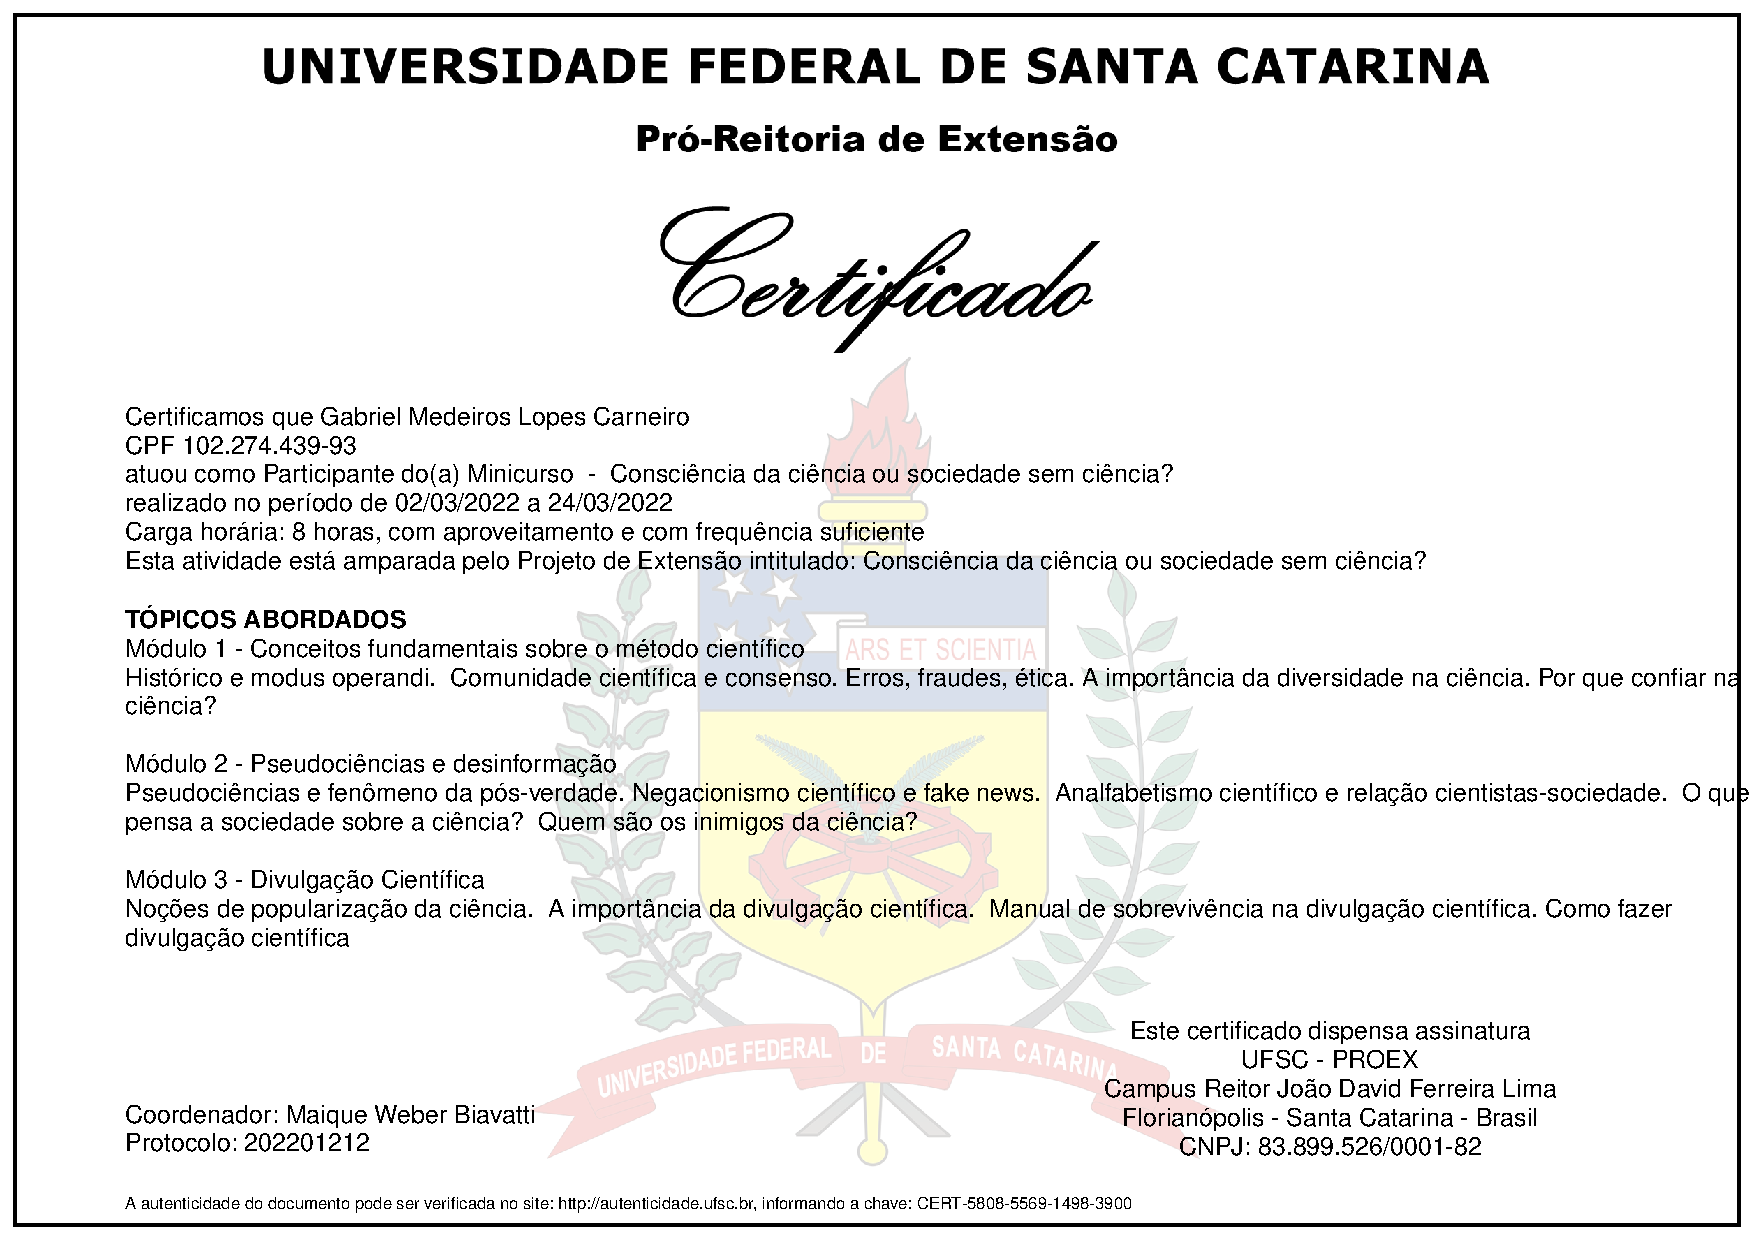
\includepdf{aftertext/minicurso-consciencia-ciencia}


\end{document}
% --------------------------------------------
% Final do documento. Não adicionar nada após.
% --------------------------------------------